\documentclass[]{standalone}
\usepackage{tikz}
\usepackage{color}
\usepackage{xcolor}
\usepackage{amssymb}
\usepackage{amsmath}
\usepackage{amsfonts}
\usepackage{mathtools}
\usepackage{xspace}
\usepackage{stmaryrd}
\usepackage[misc]{ifsym}
\usepackage{bbold}
\usepackage{etoolbox}
\usepackage{subcaption}
\usepackage{caption}
\usepackage{graphicx}

\graphicspath{{figures/}}


\usepackage[LGR, OT1]{fontenc}
\usepackage[utf8]{inputenc}

\ifcsundef{abf}{\newcommand{\wbf}{\mathbf{w}}
\newcommand{\Wbf}{\mathbf{W}}
\newcommand{\xbf}{\ensuremath{\mathbf{x}}}
\newcommand{\zbf}{\ensuremath{\mathbf{z}}}
\newcommand{\zerobf}{\mathbf{0}}
\newcommand{\h}{h}
\newcommand{\dist}{\mathrm{dist}}

\newcommand{\Acal}{\ensuremath{\mathcal{A}}}
\newcommand{\Bcal}{\ensuremath{\mathcal{B}}}
\newcommand{\Ccal}{\ensuremath{\mathcal{C}}}
\newcommand{\Dcal}{\ensuremath{\mathcal{D}}}
\newcommand{\Fcal}{\ensuremath{\mathcal{F}}}
\newcommand{\Hcal}{\ensuremath{\mathcal{H}}}
\newcommand{\Mcal}{\ensuremath{\mathcal{M}}}
\newcommand{\Ncal}{\ensuremath{\mathcal{N}}}
\newcommand{\Pcal}{\ensuremath{\mathcal{P}}}
\newcommand{\Scal}{\ensuremath{\mathcal{S}}}
\newcommand{\Tcal}{\ensuremath{\mathcal{T}}}
\newcommand{\Xcal}{\ensuremath{\mathcal{X}}}
\newcommand{\Ycal}{\ensuremath{\mathcal{Y}}}
\newcommand{\Zcal}{\ensuremath{\mathcal{Z}}}

\newcommand{\Ebb}{\ensuremath{\mathbb{E}}}
\newcommand{\Pbb}{\ensuremath{\mathbb{P}}}
\newcommand{\Rbb}{\ensuremath{\mathbb{R}}}
\newcommand{\Nbb}{\ensuremath{\mathbb{N}}}

\newcommand{\Rfrak}{\ensuremath{\mathfrak{R}}}

\newcommand{\RA}{\right\rangle}
\newcommand{\LA}{\left\langle}
\newcommand{\LB}{\left[}
\newcommand{\RB}{\right]}
\newcommand{\LC}{\left\{}
\newcommand{\LM}{\left\|}
\newcommand{\RM}{\right\|}
%\newcommand{\RC}{\right\}}
%\newcommand{\RN}{\right\vert}
\newcommand{\LN}{\left\vert}
\newcommand{\LP}{\left(}
\newcommand{\RP}{\right)}

\newcommand{\wrt}{{\it w.r.t.}\xspace}
\newcommand{\eg}{{\it e.g.}\xspace}
\newcommand{\ie}{{\it i.e.}\xspace}
\newcommand{\iid}{{\it i.i.d.}\xspace}

\newcommand{\defeq}{:=}

\DeclareMathOperator*{\EE}{\Ebb}
\DeclareMathOperator*{\PP}{\Pbb}
\DeclareMathOperator*{\argmin}{\mathrm{argmin}}
\DeclareMathOperator*{\vect}{\mathrm{vec}}
\DeclareMathOperator*{\leaky}{\mathrm{Leaky}}
\DeclareMathOperator*{\proj}{\mathrm{Proj}}

\newcommand{\Irm}{\mathrm{I}}
\newcommand{\KL}{\mathrm{KL}}
\newcommand{\KLr}{\overline{\KL}}
\newcommand{\Hell}{H^2}
\newcommand{\TV}{TV}
\newcommand{\kl}{\mathrm{kl}}
\newcommand{\W}{\mathrm{W}}
\newcommand{\Lip}{\mathrm{Lip}}

\newcommand{\D}{\Dcal}
\newcommand{\Dm}{\Dcal_{m}}
\renewcommand{\H}{\Hcal}
\newcommand{\Hb}{\overline{\Hcal}}
\newcommand{\loss}{\ell}
\renewcommand{\P}{\mathrm{P}}
\newcommand{\Q}{\mathrm{Q}}
\newcommand{\R}{\Rbb}
\newcommand{\N}{\Nbb}
\renewcommand{\S}{\Scal}
\newcommand{\Sm}{\S_m}
\newcommand{\Risk}{\text{R}}
\newcommand{\Riskhat}{\hat{\Risk}}
\newcommand{\X}{\Xcal}
\newcommand{\x}{\xbf}
\newcommand{\y}{y}
\newcommand{\Y}{\Ycal}
\newcommand{\Z}{\Zcal}
\newcommand{\z}{\zbf}
\newcommand{\varepsilonbf}{\boldsymbol{\varepsilon}}
\newcommand{\rad}{\mathdbcal{E}}
\newcommand{\DS}{\D_\S}
\newcommand{\yeast}{{\sc Yeast}\xspace}
\newcommand{\phishing}{{\sc Phishing}\xspace}
\newcommand{\mushrooms}{{\sc Mushrooms}\xspace}
\newcommand{\mnist}{{\sc MNIST}\xspace}
\newcommand{\fashion}{{\sc FashionMNIST}\xspace}
\newcommand{\indic}{\mathds{1}}

\newcommand{\OPBTest}{\normalfont\textsc{OPBTest} }
\newcommand{\OPBTrain}{\normalfont\textsc{OPBTrain} }

\newcommand{\Vhat}{\hat{V}}
\newcommand{\Bhat}{\hat{B}}
\DeclareMathOperator*{\ReLU}{\mathrm{ReLU}}

\newcommand{\Cfrak}{\ensuremath{\mathfrak{C}}}

\newcommand{\Poinc}{\texttt{Poinc}}
\newcommand{\Lsob}{\texttt{L-Sob}}
\newcommand{\Ent}{\mathrm{Ent}}
\newcommand{\Var}{\mathrm{Var}}
\DeclareMathOperator*{\Err}{\mathrm{Err}}


\let\oldQ\Q
\let\oldP\P
\renewcommand{\Q}{\orange{\oldQ}}
\renewcommand{\P}{\green{\oldP}}
}{}

%%%%%%%%%%%%%%%%%%%%%%%%%%%%%%%%%%%%%%%%%%%%%%%%%%%%%%%%%%%%%%%%%%%%%%%%%%%%%%%
% font option

\def\familydefault{\sfdefault}
\usepackage{sansmath}
\sansmath

%%%%%%%%%%%%%%%%%%%%%%%%%%%%%%%%%%%%%%%%%%%%%%%%%%%%%%%%%%%%%%%%%%%%%%%%%%%%%%%
% xcolor options
% Paul Tol's  "Vibrant" color scheme
% https://personal.sron.nl/~pault/data/colourschemes.pdf

\definecolor{blue}{HTML}{0077BB}
\definecolor{cyan}{HTML}{33BBEE}
\definecolor{green}{HTML}{009988}
\definecolor{orange}{HTML}{EE7733}
\definecolor{red}{HTML}{CC3311}
\definecolor{magenta}{HTML}{EE3377}
\definecolor{grey}{HTML}{BBBBBB}
\definecolor{blockgrey}{RGB}{245, 245, 245}

\newcommand\white[1]{\textcolor{white}{#1}}
\newcommand\black[1]{\textcolor{black}{#1}}
\newcommand\blue[1]{\textcolor{blue}{#1}}
\newcommand\cyan[1]{\textcolor{cyan}{#1}}
\newcommand\green[1]{\textcolor{green}{#1}}
\newcommand\orange[1]{\textcolor{orange}{#1}}
\newcommand\red[1]{\textcolor{red}{#1}}
\newcommand\magenta[1]{\textcolor{magenta}{#1}}
\newcommand\grey[1]{\textcolor{grey}{#1}}

%%%%%%%%%%%%%%%%%%%%%%%%%%%%%%%%%%%%%%%%%%%%%%%%%%%%%%%%%%%%%%%%%%%%%%%%%%%%%%%
\usetikzlibrary{patterns}

\begin{document}

\begin{tikzpicture}
    
    \begin{scope}
    \clip (4.73,2.13) rectangle (-0.63,-2.13);

    \draw[fill=blue,opacity=0.4] (1.95, 2.2) -- (1.95, -2.2) -- (4.7,-2.2) -- (4.7,2.2) -- cycle;
    \draw[fill=red,opacity=0.4] (-0.7, 2.2) -- (-0.7, -2.2) -- (2.0,-2.2) -- (2.0,2.2) -- cycle;

    \node[fill=red, inner sep=0.1cm] at (0,0) {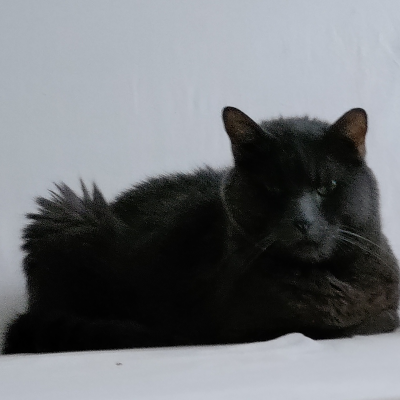
\includegraphics[scale=0.05]{supervised_cat_1.png}};
    \node[fill=red, inner sep=0.1cm] at (1.3,1) {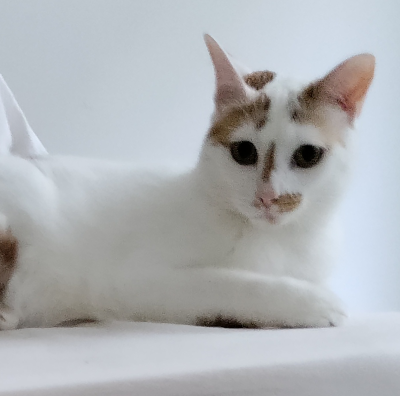
\includegraphics[scale=0.05]{supervised_cat_2.png}};
    \node[fill=red, inner sep=0.1cm] at (1.1,-0.2) {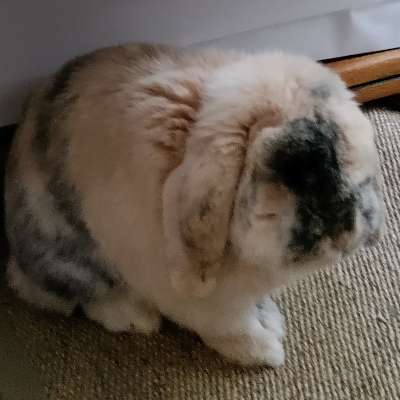
\includegraphics[scale=0.05]{supervised_cat_3.png}};
    \node[fill=red, inner sep=0.1cm] at (0.3,1.2) {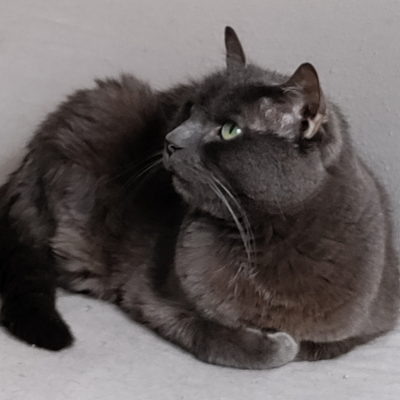
\includegraphics[scale=0.05]{supervised_cat_4.png}};
    
    \node[fill=blue, inner sep=0.1cm] at (3.5,0) {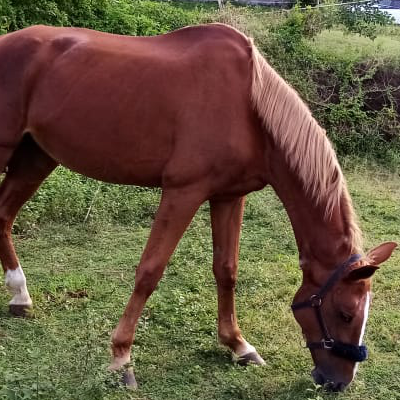
\includegraphics[scale=0.05]{supervised_horse_1.png}};
    \node[fill=blue, inner sep=0.1cm] at (2.6,1.5) {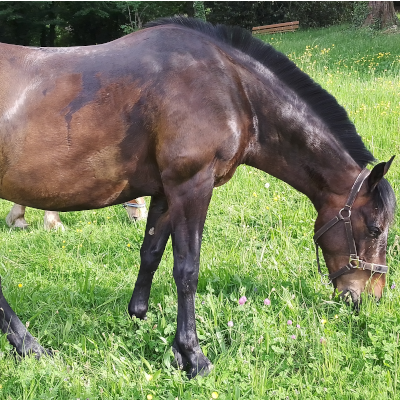
\includegraphics[scale=0.05]{supervised_horse_2.png}};
    \node[fill=blue, inner sep=0.1cm] at (4.0,-0.6) {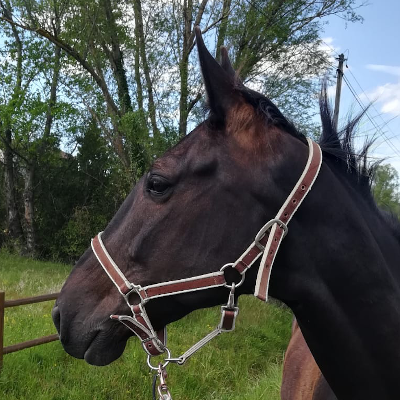
\includegraphics[scale=0.05]{supervised_horse_3.png}};
    \node[fill=blue, inner sep=0.1cm] at (2.8,-1.5) {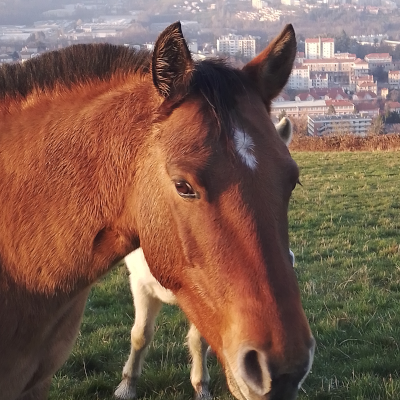
\includegraphics[scale=0.05]{supervised_horse_4.png}};
    
    \draw[line width=0.1cm, draw=black] (1.95, 2.2) -- (1.95, -2.2);
    \draw[draw=black, line width=0.05cm] (4.7,2.1) rectangle (-0.6,-2.1);
    \end{scope}
    \node[align=center] at (2.1, -2.7) {{\bf How many errors on the learning sample?}\\ 0 error!};

    
    \begin{scope}[xshift=9cm]
    \clip (4.73,2.13) rectangle (-0.63,-2.13);

    \draw[fill=blue,opacity=0.4] (1.95, 2.2) -- (1.95, -2.2) -- (4.7,-2.2) -- (4.7,2.2) -- cycle;
    \draw[fill=red,opacity=0.4] (-0.7, 2.2) -- (-0.7, -2.2) -- (2.0,-2.2) -- (2.0,2.2) -- cycle;

    \draw[line width=0.1cm, draw=black] (1.95, 2.2) -- (1.95, -2.2);

    \node[inner sep=0.1cm] at (0,0) {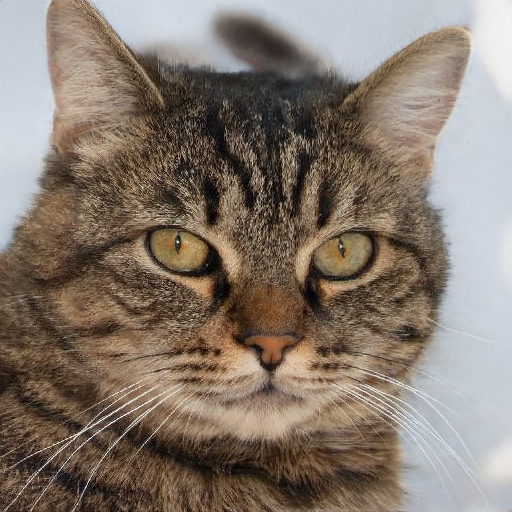
\includegraphics[scale=0.04]{new_cat_1.jpeg}};
    \node[inner sep=0.1cm] at (1.3,0.6) {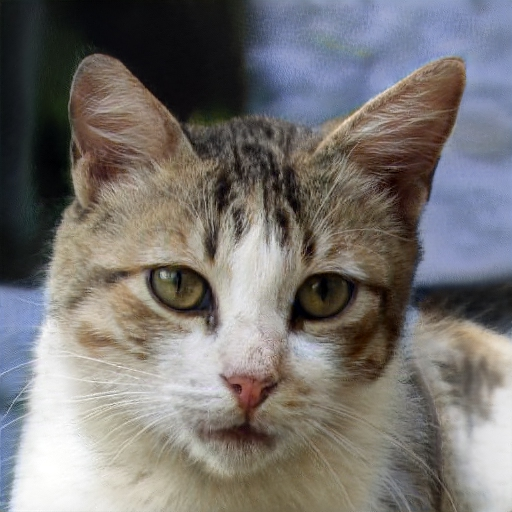
\includegraphics[scale=0.04]{new_cat_2.jpeg}};
    \node[inner sep=0.1cm] at (2.8,-1.5) {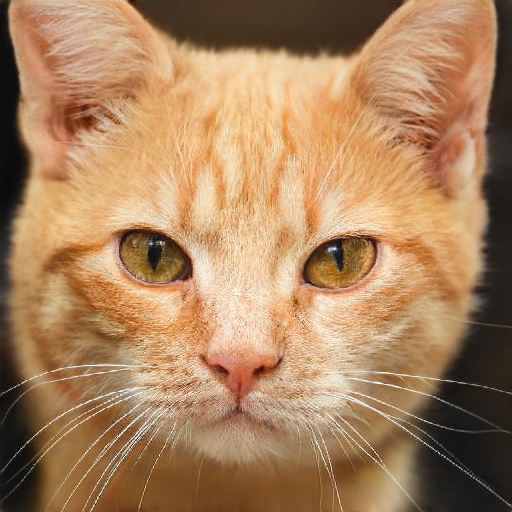
\includegraphics[scale=0.04]{new_cat_3.jpeg}};
    \node[inner sep=0.1cm] at (0.3,1.2) {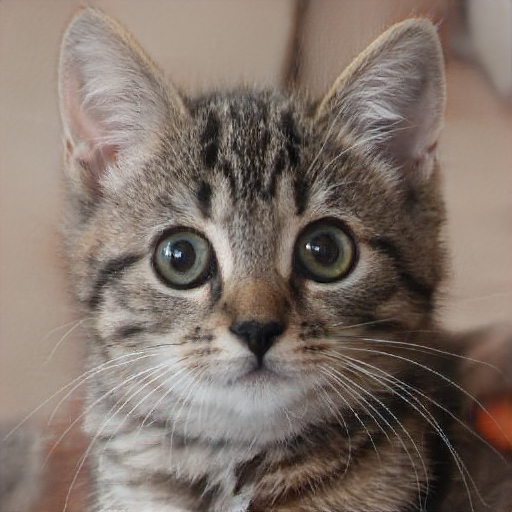
\includegraphics[scale=0.04]{new_cat_4.jpeg}};
    \node[inner sep=0.1cm] at (-0.1,-1.2) {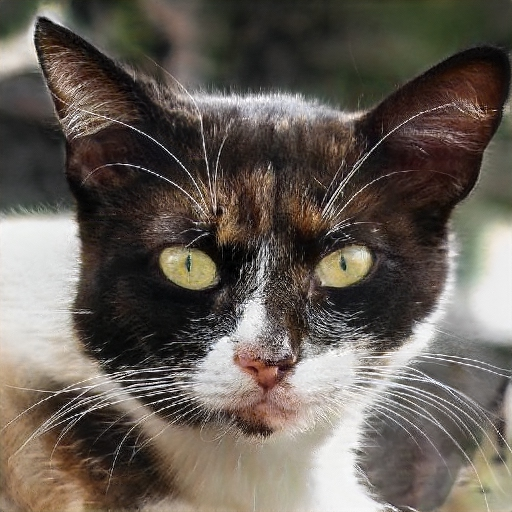
\includegraphics[scale=0.04]{new_cat_5.jpeg}};
    \node[inner sep=0.1cm] at (0.6,-1.5) {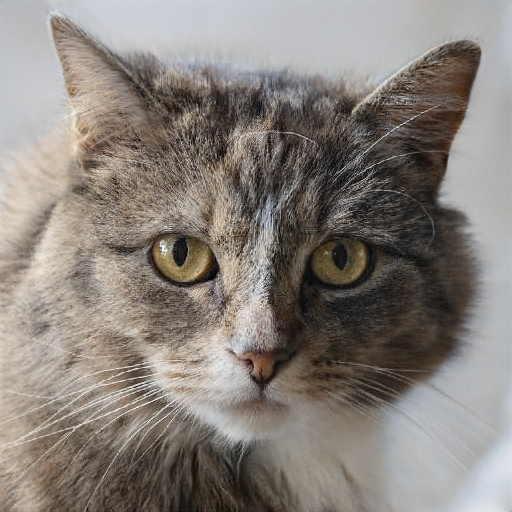
\includegraphics[scale=0.04]{new_cat_6.jpeg}};
    \node[inner sep=0.1cm] at (1.3,-1.0) {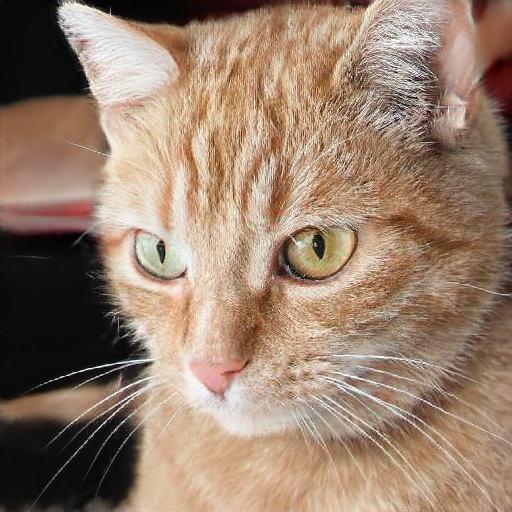
\includegraphics[scale=0.04]{new_cat_7.jpeg}};
    \node[inner sep=0.1cm] at (1.5,-1.7) {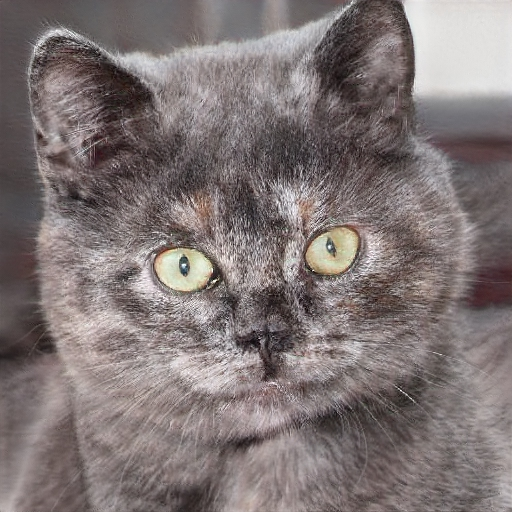
\includegraphics[scale=0.04]{new_cat_8.jpeg}};
    \node[inner sep=0.1cm] at (3.9,-1.5) {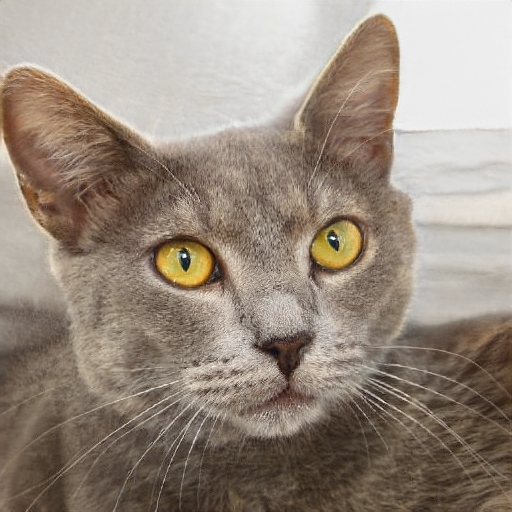
\includegraphics[scale=0.04]{new_cat_9.jpeg}};
    \node[inner sep=0.1cm] at (1.2,1.6) {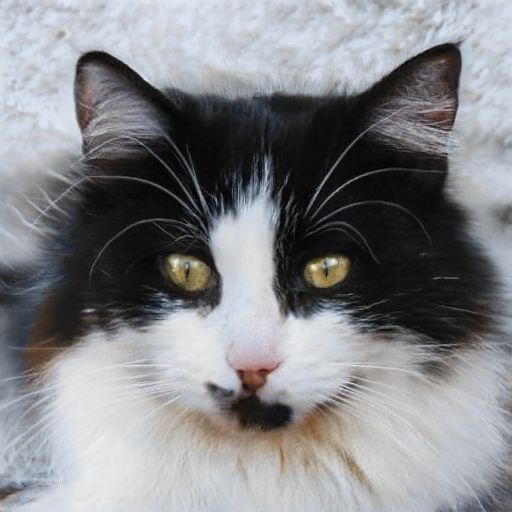
\includegraphics[scale=0.04]{new_cat_10.jpeg}};
    
    \node[inner sep=0.1cm] at (3.5,0) {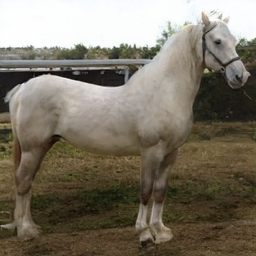
\includegraphics[scale=0.08]{new_horse_1.jpeg}};
    \node[inner sep=0.1cm] at (2.6,1.5) {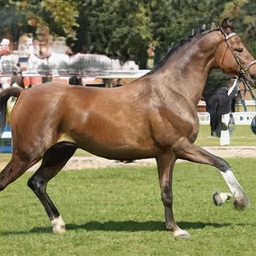
\includegraphics[scale=0.08]{new_horse_2.jpeg}};
    \node[inner sep=0.1cm] at (4.0,-0.6) {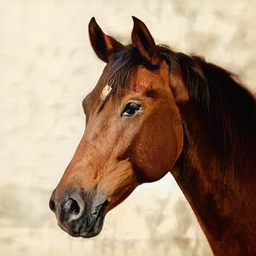
\includegraphics[scale=0.08]{new_horse_3.jpeg}};
    \node[inner sep=0.1cm] at (1.1,-0.2) {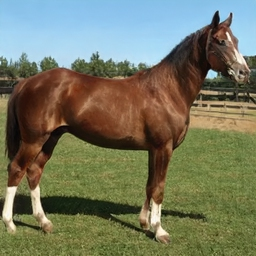
\includegraphics[scale=0.08]{new_horse_4.jpeg}};
    \node[inner sep=0.1cm] at (2.6,-0.5) {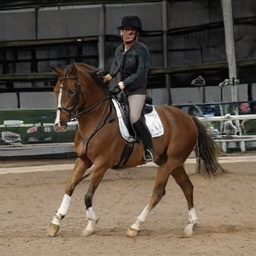
\includegraphics[scale=0.08]{new_horse_5.jpeg}};
    \node[inner sep=0.1cm] at (2.4,0.3) {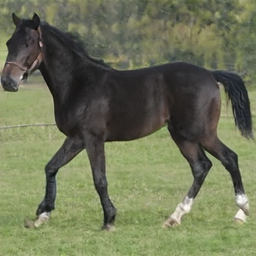
\includegraphics[scale=0.08]{new_horse_6.jpeg}};
    \node[inner sep=0.1cm] at (3.0,0.7) {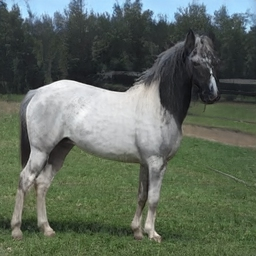
\includegraphics[scale=0.08]{new_horse_7.jpeg}};
    \node[inner sep=0.1cm] at (4.0,0.7) {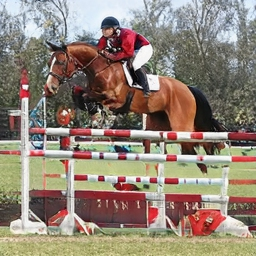
\includegraphics[scale=0.08]{new_horse_8.jpeg}};
    \node[inner sep=0.1cm] at (3.4,1.4) {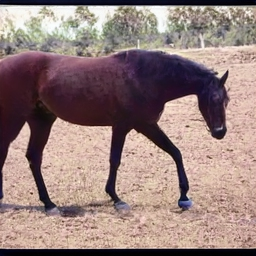
\includegraphics[scale=0.08]{new_horse_9.jpeg}};
    \node[inner sep=0.1cm] at (4.0,1.7) {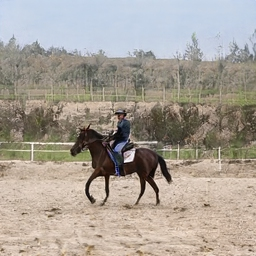
\includegraphics[scale=0.08]{new_horse_10.jpeg}};
    \draw[draw=black, line width=0.05cm] (4.7,2.1) rectangle (-0.6,-2.1);
    \end{scope}
    
    \draw[draw=red, line width=0.1cm] (11.8,-1.50) circle (0.55cm);
    \draw[draw=red, line width=0.1cm] (12.9,-1.50) circle (0.55cm);
    \draw[draw=blue, line width=0.1cm] (10.1, -0.2) circle (0.55cm);
    
    \node[align=center] at (11.1, -2.7) {{\bf How many errors on new examples?}\\ 3 errors\dots};
    
\end{tikzpicture}
\end{document}